\label{chap:main_work}
In this chapter, the main contents of the thesis work are represented.
Figure \ref{fig:framework} shows the framework of the memory power
optimization process using the simulated annealing algorithm.
There are two kinds of input for the simulated annealing algorithm.
One is the input data related to the optimization problem.
These raw data is recorded in different text files but their data
structure is not suitable for the simulate annealing algorithm.
Thus, a proper input data organization is defined and a parsing
method is used to transform the raw data into this data organization.
Section \ref{sec:input_organ} discusses the input data organization
and the parsing method in detail.
The other kind of input for the algorithm is the algorithm parameter.
The discussion of these parameters are made in Section.....which also
introduce the design of the simulated in detail.
\begin{figure}[H]
	\begin{center}
		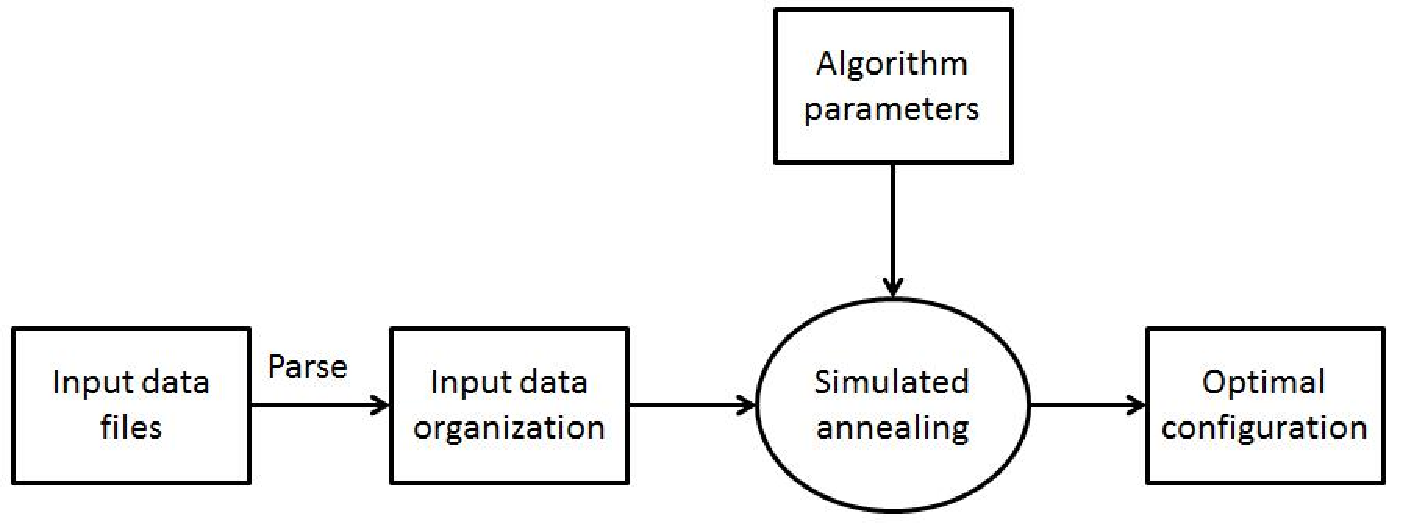
\includegraphics[width=0.7\textwidth]{optim_framework}
		\caption{Framework of The Simulated Annealing for Memory Power Optimization}
		\label{fig:framework}
	\end{center}
\end{figure}
	\section{Input data organization}
	\label{sec:input_organ}
	As discussed in Section \ref{sec:memory_partition}, the formal
	power model requires the parameters that are relevant to the
	memory types, the application profiles and the interconnect.
	Thus, these parameters are the input data to the simulated
	annealing algorithm.
	Since the object oriented programming is planned to be used for
	the implementation of the simulated annealing, the parameters
	that are related to the same item can be grouped together into
	one class. For example, the physical parameters that are
	relevant to the memory type can reside in the memory class.
	Figure \ref{fig:uml} shows the input parameters
	organization in the form of the UML class diagram.

	\begin{figure}[htb]
		\begin{center}
			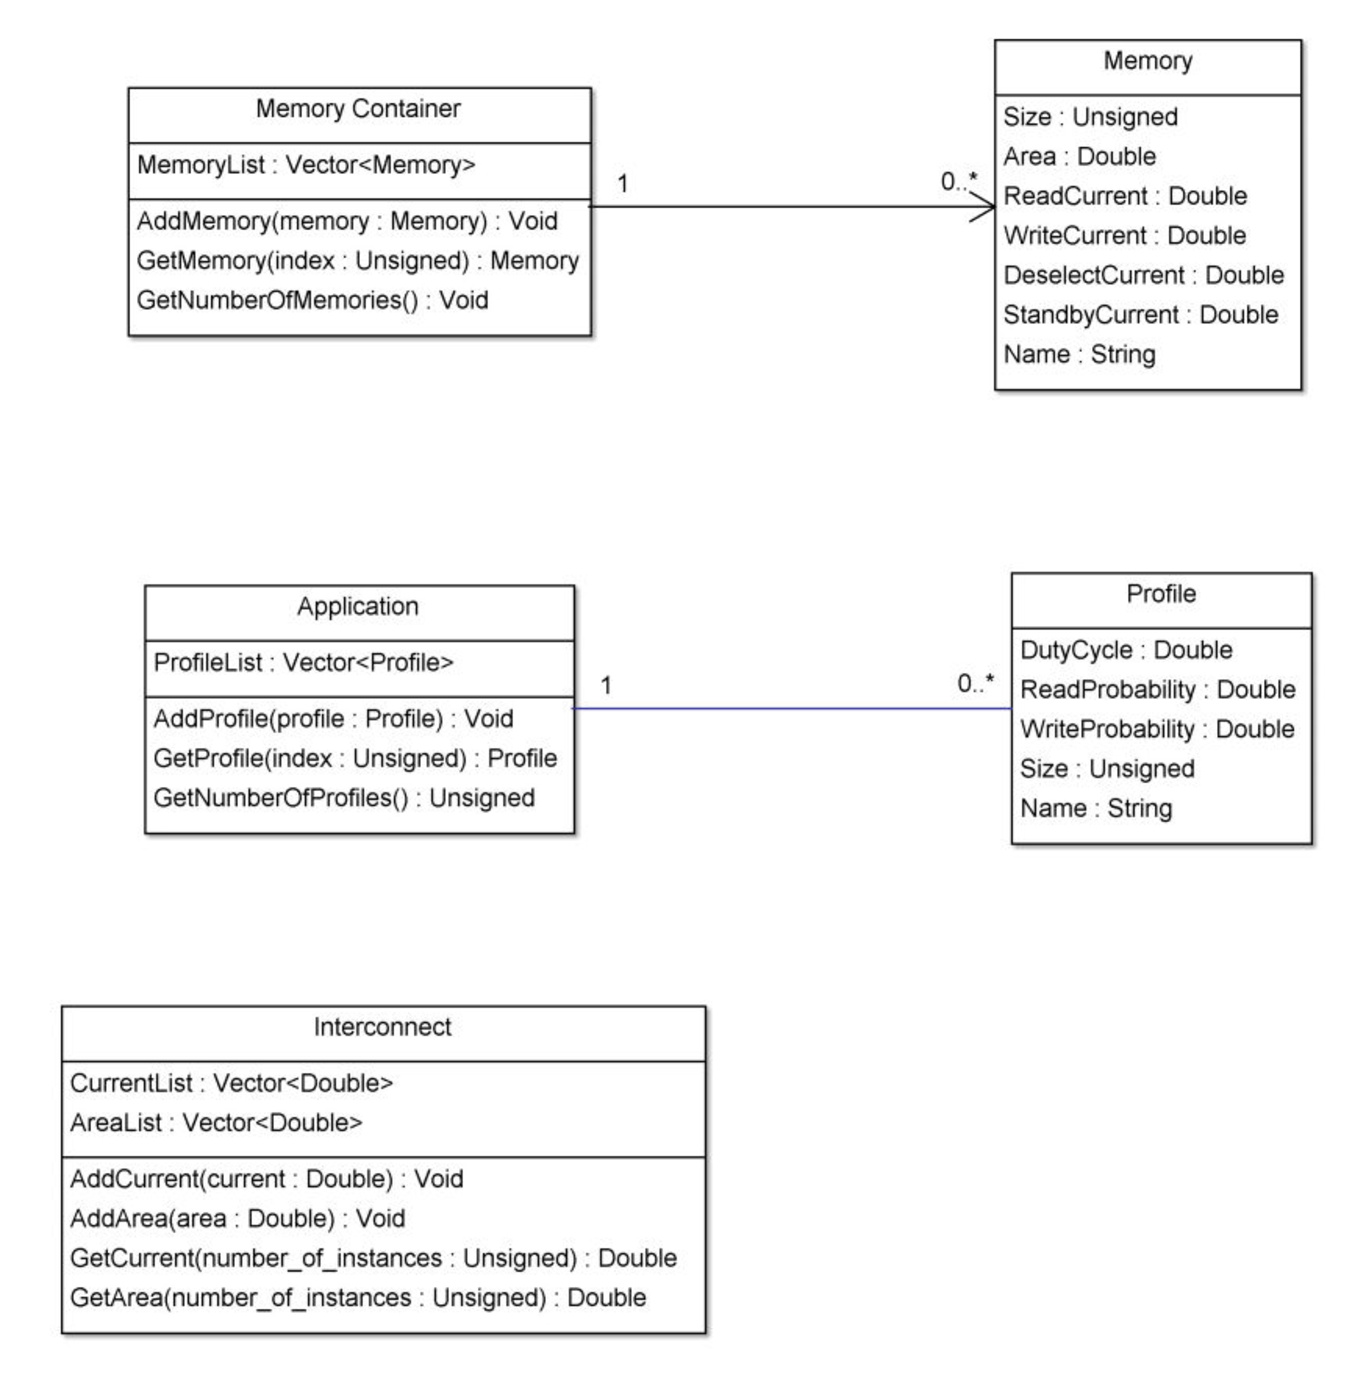
\includegraphics[width=0.7\textwidth]{uml_class}
			\caption{Input Parameter Organization in UML Diagram}
			\label{fig:uml}
		\end{center}
	\end{figure}
	
	The memory class includes all its parameters that are used in the
	formal power model.  Since there are a set of memory types in the
	power model, a set of objects of the memory class will be created in
	the simulated annealing algorithm as well. Thus the memory container
	class is defined to store these memory objects.
	And the algorithm can also retrieve the required objects and the
	total number of memory objects through the corresponding operations
	in the memory container class.
	The profile class and the application class are defined similarly
	to the memory class and the memory container class respectively.
	However, the interconnect is different. It uses two lists to store the
	current and area parameters whose value are dependent on the total
	number of instances. These parameters can be also retrieved by the
	simulated annealing algorithm through the corresponding operations
	defined in the interconnect class.
	\begin{figure}[htb]
		\begin{center}
			\subfloat[][]
			{
				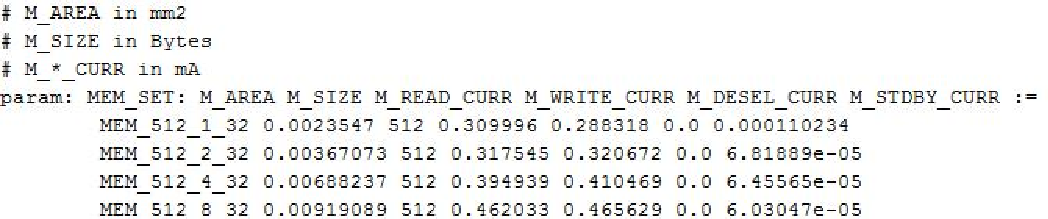
\includegraphics[width=0.7\textwidth]{mem_data}
				\label{subfig:mem_data}
			}
			\qquad
			\subfloat[][]
			{
				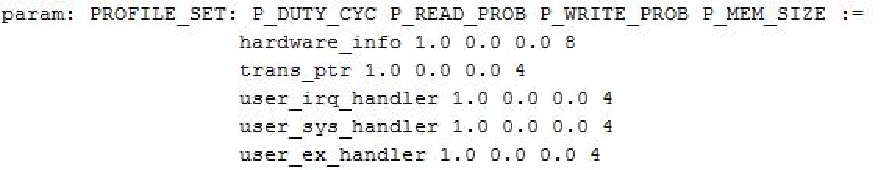
\includegraphics[width=0.7\textwidth]{profile_data}
				\label{subfig:profile_data}
			}
			\qquad
			\subfloat[][]
			{
				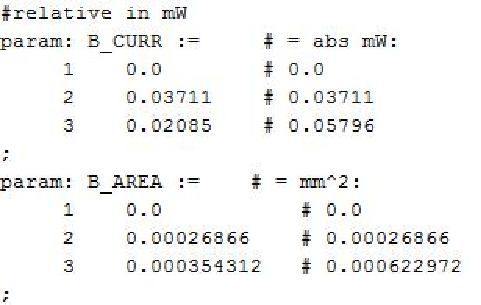
\includegraphics[width=0.4\textwidth]{ic_data}
				\label{subfig:ic_data}
			}
		\end{center}
		\caption{Fragments of The Input Parameter Data Files \cite{Strobel2016}}
		\label{fig;input_data}
	\end{figure}

	In this thesis work, the same data sets provided in \cite{Strobel2016}
	are used as the references for the input parameters data of the simulated
	annealing algorithm. These input parameters data are recorded in multiple
	plain text data files. Figure \ref{fig;input_data} represents some fragments
	of these data files. Figure \ref{subfig:mem_data} is the fragment of the
	memory data file. Figure \ref{subfig:profile_data} shows the fragment of the
	application profile data file and Figure \ref{subfig:ic_data} is the
	fragment of the interconnect data file. In order to group the data
	contained in these files into the designed input data organization, a
	parsing method is used. The basic idea of the parsing method is to read the
	plain text file line by line. The required data is extracted and the
	unnecessary data is discarded. Since the data file is text-based,
	the required data are converted into the corresponding data type during the
	extraction.

	\setlength{\textfloatsep}{0.2cm}
\begin{algorithm2e}[H]
	\KwIn{a memory\textbackslash profile data file, a memory container\textbackslash application object}
	\KwOut{void}
	\While{not end of the file}
	{
		read one line\;
		\If{relevant data is contaied in the line}
		{
			extract the data\;
			convert the extracted data into the corresponding type\;
			create a memory\textbackslash profile object based on the converted data\;
			add the created object into the list of the memroy container\textbackslash application object\;
		}
	}
	\caption{Parse Memory\textbackslash Profile Data File}
	\label{algo:mem_profile_parser}
\end{algorithm2e}
\setlength{\textfloatsep}{0.2cm}
	
	Algorithm \ref{algo:mem_profile_parser} is the pseudo-code of
	the parsing method for the memory and profile data files. If the method is
	used to parse the memory data file, it first reads one line of the file text.
	Then it checks whether there is the relevant data contained in the line or not.
	If there is no data, the the algorithm continues reading the next line.
	Otherwise, the relevant data is extracted and converted into the corresponding
	data type.
	It can be seen from the file fragment in Figure \ref{subfig:mem_data}, all the
	parameters data related to one memory type are listed in one single line.
	Thus, a memory object can be created based on the retrieved and converted data
	for one line. And the created object is added to the list in the memory container
	object. The same parsing step is repeated until the method reaches the end of
	the file. The parsing process of the application profile data file is similar
	to the parsing of the memory data file.
	The only differences are that it deals with the profile data file and the
	profile objects are created and added to the list of the application object.
	However, the parsing method of the interconnect data file is modified slightly.
	Algorithm \ref{algo:ic_parser} shows the pseudo-code of the parsing method for
	the interconnect data file.
	From the file fragment in Figure \ref{subfig:ic_data} it can be seen that there
	are two parts in the interconnect data file.
	The first part contains the interconnect current data while the other part
	records the interconnect area data. Thus, after the extracted data is converted,
	the parsing method needs to check whether the data is related to the current or
	the area. Then the data is added to the corresponding list of the interconnect
	object.
	
	\setlength{\textfloatsep}{0.2cm}
\begin{algorithm2e}[H]
	\KwIn{an interconnect data file, an interconnect object}
	\KwOut{void}
	\While{not end of the file}
	{
		read one line\;
		\If{relevant data is contaied in the line}
		{
			extract the data\;
			convert the extracted data into the corresponding type\;
			\eIf{is current data}
			{
				add the converted data into the current list of the interconnect object\;
			}
			{
				add the converted data into the area list in of interconnect object\;
			}
		}
	}
	\caption{Parse Interconnect Data File}
	\label{algo:ic_parser}
\end{algorithm2e}
\setlength{\textfloatsep}{0.2cm}
	
	\section{Simulated annealing design flow}
	\label{sec:sa_design_flow}
	The major design of the simulated annealing for the memory power optimization is
	the algorithm structure. Before the design details are introduced, an abstract
	design flow of the simulated annealing algorithm is provided in Figure
	\ref{fig:sa_framwork}. From the figure it can be seen that the algorithm is
	consisted of three parts.
	In the initialization of the algorithm, $S_{curr}$ is
	the current solution. It is set to an initial solution $S_{0}$. $C_{curr}$ is the
	cost of $S_{curr}$ and it is calculated according to $S_{0}$. The temperature
	$T$ is set to an initial value $T_{0}$.
	The second part of the algorithm is the inner loop. $S_{neigh}$ is the neighboring
	solution generated by the method $Neighbor()$ based on $S_{curr}$. Its cost
	$C_{neigh}$ is calculated by the cost function $Cost()$. Then the metropolis
	criterion $Metropolis()$ is performed to update $S_{curr}$ according
	to $C_{curr}$ and $C_{neigh}$.
	$Termination_{inner}$ is the termination condition for the inner loop.
	The last part of the algorithm is the outer loop. $CoolingSchedule$ is used to
	decrease $T$. $Termination_{inner}$ is the termination condition for the outer loop.
	\begin{figure}[htb]
		\begin{center}
			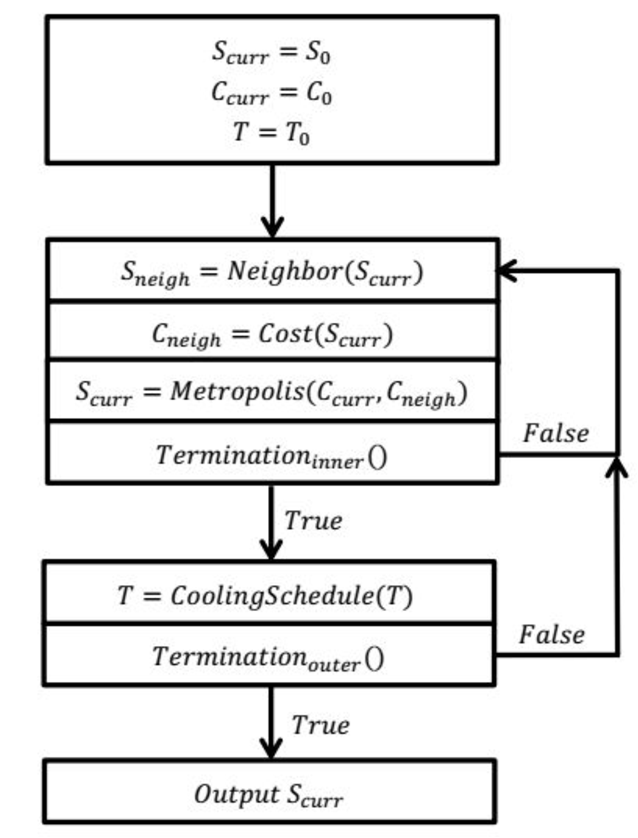
\includegraphics[width=0.7\textwidth]{sa_framework}
			\caption{Simulate Annealing Design Flow}
			\label{fig:sa_framwork}
		\end{center}
	\end{figure}	

	The design of the simulated annealing should contains the answers of Question
	\ref{ques:1} to \ref{ques:7}. To enhance the readability of the rest of this
	chapter, the design details discussed will answer these questions sequentially.
	By providing an approach for each of these questions, the design for the
	simulated annealing algorithm is completed.
	\begin{enumerate} [\text{Question} 1:]
		\item What is the representation of solutions?
		\label{ques:1}
		\item How to generate neighboring solutions?
		\label{ques:2}
		\item What is the cost function?
		\label{ques:3}
		\item How to implement the metropolis criterion?
		\label{ques:4}
		\item What is the cooling schedule?
		\label{ques:5}
		\item How to determinate the initial solution and the initial temperature?
		\label{ques:6}
		\item How to terminate the inner loop and the outer loop?
		\label{ques:7}
	\end{enumerate}

	\section{Approach 1}
	\label{sec:stage_1}
	This approach is to seek for the optimal memory allocation and the binding of profiles
	simultaneously. Section \ref{subsec:design_1} gives the answers of the design
	questions and Section \ref{subsec:problem_1} discusses the problems of this approach.
		\subsection{Design process}
		\label{subsec:design_1}
		Question \ref{ques:1}: What is the representation of solutions?
		
		As discussed in Section \ref{sec:memory_partition}, the result of the memory
		partitioning process is a configuration for the memory system.
		The solution provided by the simulated annealing algorithm should correspond to the memory configuration.
		According to this, solutions of the simulated annealing algorithm are defined as following. A solution is in the form of an integer vector that are divided into two parts. The first part of the vector corresponds to the allocation of memories.
		Each element in this part is the number of memory instances of the corresponding
		memory type.
		The second part of the vector contains the information about the binding of profiles. Each element in this part is the index of the memory type to which the corresponding
		profile is bound.
		Therefore, the vector size is the sum of the number of memory types and the number of profiles.
		To be clear, the first part of the vector is called the allocation part of
		the solution while the second part of the vector is called the binding part
		of the solution. The vector size is called solution length.
		Figure \ref{fig:solu_exam_1} shows a solution example with two memory types and three application profiles.
		In the allocation part of the solution, one instance is allocated for both memory types.
		In the binding part, profile 0 is bound to memory type 0.
		Profile 1 and 2 are both bound to memory type 1.
		\begin{figure}[h]
			\begin{center}
				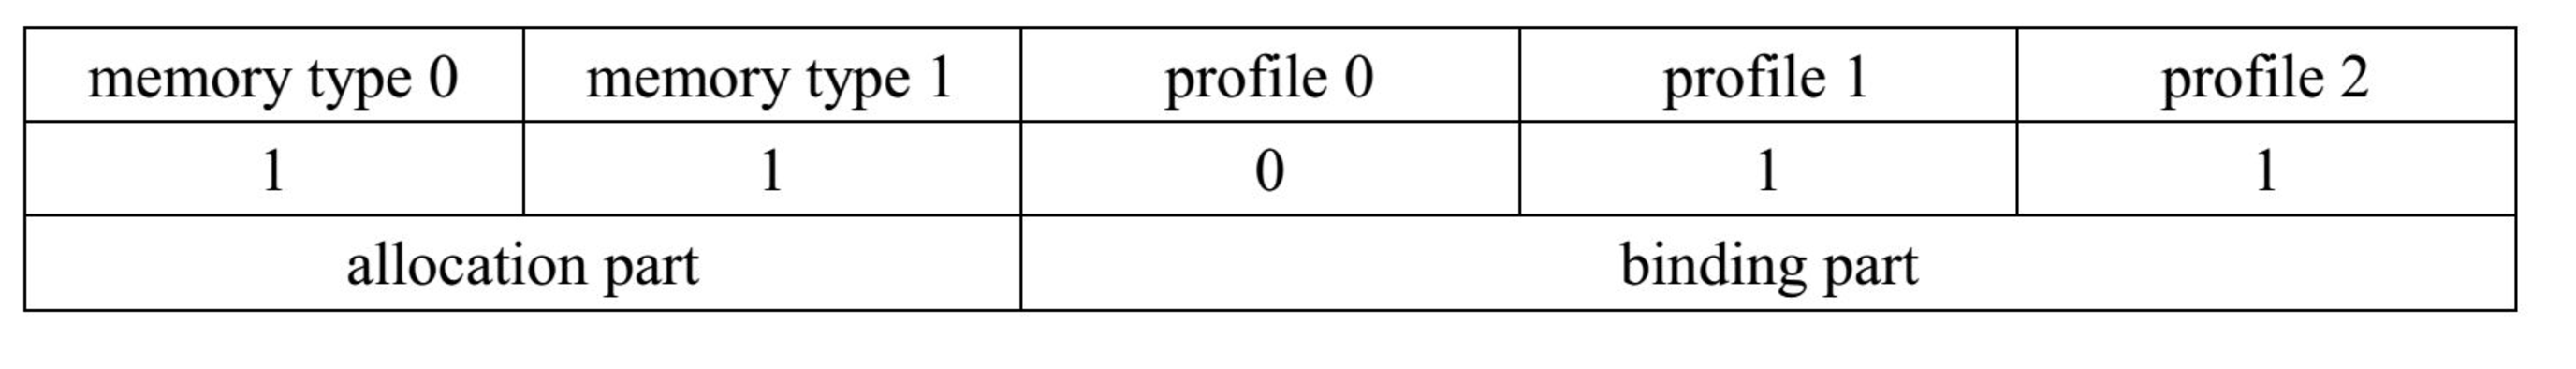
\includegraphics[width=0.7\textwidth]{solution_example_1}
				\caption{A Solution Example}
				\label{fig:solu_exam_1}
			\end{center}
		\end{figure}

		Question \ref{ques:2}: How to generate neighboring solutions?
		
		According to the solution representation, the neighborhood solutions are described
		as following. 
		A neighboring solution is a vector with same length of the
		original solution. Only one element in the vector is different from the
		original solution.
		Figure \ref{fig:neigh_solu_exam_1} shows an example of neighboring solutions.
		The original solution is the same in Figure \ref{fig:solu_exam_1}.
		In neighboring solution 1, two memory instances are allocated for memory type 0
		while only one instance is allocated in the original solution.
		The rest elements of neighboring solution 1 are the same with the original solution.
		In neighboring solution 2, the only difference to the original solution is that
		profile 2 is bound to memory type 0.
		\begin{figure}[h]
			\begin{center}
				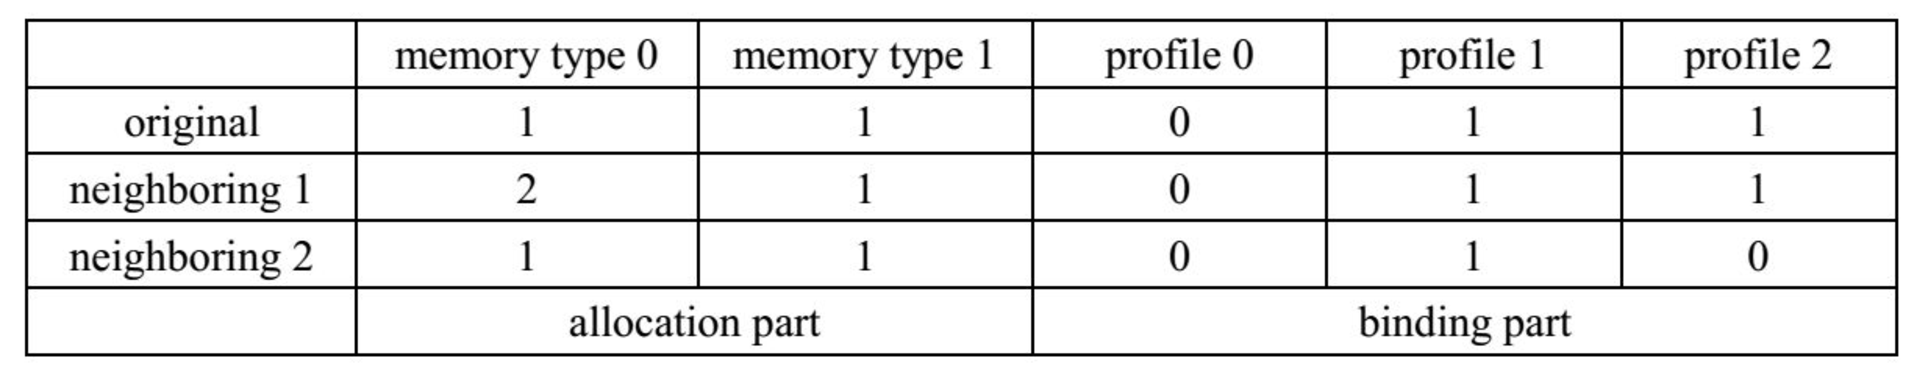
\includegraphics[width=0.7\textwidth]{neigh_example_1}
				\caption{Neighboring Solutions Example}
				\label{fig:neigh_solu_exam_1}
			\end{center}
		\end{figure}

		In this approach, the basic idea of $Neighbor()$ is to modify one element from the
		current solution. When generating neighboring solutions, the constraints of the formal power model should be taken into consideration.
		To ensure the constrain 1 and 3, the modification of the chosen element is limited in a
		range. As the solution is consisted of two different parts, the ranges of this two parts are also different.
		Let $Range_{\alpha}$ and $Range_{\beta}$ denote the modification ranges for the allocation part
		and the binding part respectively.
		The lower bound of $Range_{\alpha}$ is 0. The upper bound of $Range_{\alpha}$ is computed as following.
		Let $mems_{total}$ denote the total number of memory instances in the current solution.
		Suppose element $i$ in the allocation part is selected to be modified.
		Let $mem_{i}$ denotes the number of instances of memory type $i$ in the current solution.		
		Then the upper bound of $Range_{\alpha}$ equals $(mems_{max}-mems_{total}+mem_{i})$.
		$mems_{max}$ is the predefined constraint in the Equation \ref{equa:constraint_1}.
		For $Range_{\beta}$, its lower bound is 0.
		Let $Num_{memtype}$ denote the number of memory types.
		The upper bound of $Range_{\beta}$ is $(Num_{memtype}-1)$.
		
		Algorithm \ref{algo:neighbor_1} is the pseudo-code of $Neighbor()$.
		In the algorithm, there is another method $ConstraintsCheck()$.
		This method is used to examine whether the generated neighboring solutions satisfy the
		constrain 2 (Equation \ref{equa:constraint_2}) and constraint 4
		(Equation \ref{equa:constraint_4}) of the power model.
		Algorithm \ref{algo:constrain_check_1} shows the pseudo-code of $ConstraintsCheck()$.
		$ConstraintsCheck()$ first checks whether the area constraint $area_{max}$ is satisfied
		or not.
		$area_{total}$ is the total area consumed by the memory instances and the interconnect.
		Then for each memory type, $ConstraintsCheck()$ examines whether enough memory space is
		provided for the profiles that are bound to the memory type.
		\setlength{\textfloatsep}{0.2cm}
\begin{algorithm2e}[t]
	\KwIn{$S_{curr}$}
	\KwOut{$S_{neigh}$}
	create a new solution $S_{neigh}$\;
	\While{ConstraintsCheck($S_{neigh}$) is false}
	{
		$S_{neigh}=S_{curr}$\;
		randomly selecte an element $element_{i}$ in $S_{neigh}$\;
		\eIf{$element_{i}$ is in the allocation part}
		{
			$element_{i}$ = Rondom number in $Range_{\alpha}$\;
		}
		{
			$element_{i}$ = Rondom number in $Range_{\beta}$\;
		}
	}
	\Return $S_{neigh}$ \;
	\caption{$Neighbor()$}
	\label{algo:neighbor_1}
\end{algorithm2e}
\setlength{\textfloatsep}{0.2cm}
		\setlength{\textfloatsep}{0.2cm}
\begin{algorithm2e}[h]
	\KwIn{$S_{neigh}$}
	\KwOut{a boolean value}
		compute $area_{total}$\;
		\eIf{$area_{total}>area_{max}$}
		{
			\Return false\;
		}
		{
			\ForEach {memory type $mt_{i}$}
				{
					find all profiles bound to $mt_{i}$\;
					compute the memory $mem_{required}$ required by these profiles\;
					compute the memory $mem_{provided}$ provided by $mt_{i}$\;
					\If{$mem_{provided}<mem_{required}$}
					{
						\Return false\;
					}
				}
				\Return true\;
		}
	\caption{$ConstraintsCheck()$}
	\label{algo:constrain_check_1}
\end{algorithm2e}
\setlength{\textfloatsep}{0.2cm}

		Question \ref{ques:3}: What is the cost function?
		
		Because the solution of the simulated annealing algorithm corresponds to the
		memory configuration, the solution cost $C$ is defined as the average power
		consumption of the configuration. The cost function $Cost()$ is designed
		based on the formal power model that is introduced in Section
		\ref{sec:memory_partition}. All the relevant parameter data required by the
		power model can be fetched from the input parameter organization.
	
		Question \ref{ques:4}: How to implement the metropolis criterion?
	
		The procedure of the metropolis criterion is straightforward and its
		implementation is illustrated in Algorithm \ref{algo:metropolis}.
		Because the goal of the power memory optimization is to reduce the
		power consumption, the solution with lower cost is considered as the
		better one in the metropolis criterion.
		A random real number $R$ is generated by the method $Random()$.
		This method only generates real numbers that are uniformly distributed in the
		range of 0 to 1 due to that $R$ is compared with the acceptance probability
		$P_{accept}$.
	
		\setlength{\textfloatsep}{0.2cm}
\begin{algorithm2e}[h]
	\KwIn{$C_{curr},C_{neigh},T$}
	\KwOut{void}
	\eIf{$C_{curr} \leq C_{neigh}$}
	{
		$S_{curr}=S_{neigh}$\;
		$C_{curr}=C_{neigh}$\;
	}
	{
		$P_{accept}=\exp{\left( -\frac{C_{neigh}-C_{curr}}{T} \right)}$\;
		$R = Random()$\;
		\If{$R \leq P_{accept}$}
		{
			$S_{curr}=S_{neigh}$\;
			$C_{curr}=C_{neigh}$\;	
		}
	}
	\caption{Metropolis Criterion Precedure}
	\label{algo:metropolis}
\end{algorithm2e}
\setlength{\textfloatsep}{0.2cm}
	
		Question \ref{ques:5}: What is the cooling schedule?
		
		For the cooling schedule, the temperature $T$ is linearly reduced with a fixed
		cooling ration $R_{cool}$.
		Equation \ref{equa:cooling_sche} is the design of $CoolingSchedule()$, where
		$N$ is the number of outer loop iterations.
		Obviously, the value of the $R_{cool}$ should be a positive real number and
		it must be less than 1 in order to decrease $T$.
		However, it is a non-trivial task to determine a proper value for $R_{cool}$
		In this approach, the value of $R_{cool}$ is set to 0.9 first and it can be
		adjusted base on experiments.
		\begin{equation}
		\label{equa:cooling_sche}
			T_{N+1}=R_{cool} \cdot T_{N}
		\end{equation}
		
		Question \ref{ques:6}: How to determinate the initial solution and the
		initial temperature?
		
		The initial solution $S_{0}$ of the simulated annealing algorithm can be set
		to a given solution manually.
		In this approach, $S_{0}$ is set as following.
		Only one larger enough memory instance is allocated so that all application
		profiles can be bound to it.
		
		For the determination of the initial temperature $T_{0}$, the initial acceptance
		probability $P_{0}$ is defined.
		As Kirkpatrick et al. propose in the original article,
		$P_{0}$ is the expected acceptance probability of worser solutions at $T_{0}$
		\cite{10.2307/1690046}.
		In this approach, $T_{0}$ is computed by Equation \ref{equa:t_0_1} based
		on the metropolis criterion (Equation \ref{equa:metropolis_equation}).
		In Equation \ref{equa:t_0_1}, $\left( C_{neigh}-C_{curr} \right)_{max}$
		is the maximum cost difference between a worser neighboring solution and the current
		solution.
		It can be measured by generating a set of worser neighboring solutions of the
		current solution randomly.
		The value of $P_{0}$ should be a positive real number less than 1.
		It should be close to 1 because the neighboring solutions are randomly
		accepted at $T_{0}$.
		$P_{0}$ is set to 0.9 in this approach and it can be adjusted based on experiments.
		\begin{equation}
		\label{equa:t_0_1}
			T_{0}= - \frac{\left( C_{neigh}-C_{curr} \right)_{max} }{ln{P_{0}}}
		\end{equation}
		
		Question \ref{ques:7}: How to terminate the inner loop and the outer loop?
		
		For the inner loop of the simulated annealing algorithm, the
		number of iterations is limited to a maximum number $Max_{iteration}$.
		During the execution of the inner loop, the number of iterations
		$Num_{iteration}$ is counted.
		When $Num_{iteration}$ becomes larger than $Max_{iteration}$, the inner
		loop terminates.
		The value of $Max_{iteration}$ is related to the size of the
		neighborhood $Size_{neighbor}$. $Size_{neighbor}$ is defined as the number
		of neighboring solutions of the current solution.
		In this approach, it is fixed to the solution length for simplification.
		Equation \ref{equa:iteration_innerloop} illustrates how to calculate the value of $Max_{iteration}$.
		From the equation it can be seen that $Max_{iteration}$ is proportional
		to $Size_{neighbor}$ with a factor $F_{iteration}$.
		The value of $F_{iteration}$ should be a positive real number.
		In this approach, $F_{iteration}$ is set to be 1 and it can also be modified based on
		experiments.
		\begin{equation}
		\label{equa:iteration_innerloop}
			Max_{iteration}=F_{iteration} \cdot Size_{neighbor}
		\end{equation}
		
		For the outer loop termination, a low temperature limit $T_{low}$ is defined.
		When the temperature $T$ is decreased to $T_{low}$, the outer loop terminates.
		The determination of $T_{low}$ is similar to the determination of $T_{0}$.
		$P_{low}$ is defined as the expected acceptance probability at $T_{low}$.
		Then $T_{low}$ is computed according to Equation \ref{equa:t_low_1}.
		In the equation, $\left( C_{neigh}-C_{curr} \right)_{min}$ is the minimum cost
		difference between a worser neighboring solution and the current solution.
		It can be measured by generating a set of worser neighboring solutions randomly
		as well. The value of $P_{low}$ should be a positive real number close to 0
		because the simulated annealing algorithm behaves like the local search algorithm
		at $T_{low}$. The worser neighboring solutions are seldom accepted.
		In this approach, the value of $P_{low}$ is set to 0.1 and it can be adjusted
		base on experiments.
	\begin{equation}
	\label{equa:t_low_1}
		T_{low}= - \frac{\left( C_{neigh}-C_{curr} \right)_{min}}{ln{P_{low}}}
	\end{equation}	
	
	\subsection{Problem discussion}
	\label{subsec:problem_1}
	The problems
	
	\section{Stage 2}
	\label{sec:stage_2}
	From the approach discussed in Section \ref{sec:stage_1}, finding the optimal allocation and
	the binding at the same time seems to be problematical.
	In this approach, the memory power optimization is divided into two related sub-processes.
	One is the optimization for the allocation and the other one is the optimization for the
	binding. The allocation optimization is dependent on the result of the binding optimization.
	The simulated annealing algorithm is used for each of the sub-processes.
	To be simplified, let $SA_{\alpha}$ denote the simulated annealing algorithm for the
	allocation optimization and let $SA_{\beta}$ denote the simulated annealing algorithm
	for the binding optimization. Then the basic idea of this approach is to use $SA_{\beta}$
	as the object function of $SA_{\alpha}$.
	
	In the approach discussed in Section \ref{sec:stage_1}, the solution for the simulated annealing
	algorithm is consisted of the allocation part and the binding part. In this approach, the
	allocation part is defined as the solution of $SA_{\alpha}$ while the binding part is defined
	as the solution of $SA_{\beta}$.
	
	The neighborhood structures of $SA_{\alpha}$ and $SA_{\beta}$ are describe as following.
	For both $SA_{\alpha}$ and $SA_{\beta}$, the neighboring solutions are define as the same
	in Section \ref{sec:stage_1}. The neighboring solutions are one element different from the
	current solution. However, the methods to generate neighboring solutions are different.
	Let $Neighbor_{\alpha}$ and $Neighbor_{\beta}$ denote the generating method of $SA_{\alpha}$
	and $SA_{\beta}$ respectively.
	Instead of modifying the chosen element value according to a limited range, $Neighbor_{\alpha}()$
	increases or decreases the value of the selected element by 1. The probabilities of the increase
	and decrease are both 0.5.But if the original value of the chosen element is 0, it can only be
	increased because the element value should be positive.
	Algorithm \ref{algo:neighbor_alfa} is the pseudo-code for
	$Neighbor_{\alpha}()$. In the algorithm, $S_{\alpha,curr}$ is the current solution of
	$SA_{\alpha}$ and $S_{\alpha,neigh}$ is its neighboring solution. Similar to the Algorithm
	\ref{algo:neighbor_1}, the method $ConstraintsCheck_{\alpha}()$ is used to check whether the
	generated neighboring solutions satisfy the constraints.
	In this approach, the constraints of the power model is divided to two parts as well.
	Constraint 1 and 2 are grouped together and they are called $Constraint_{\alpha}$.
	Constraint 3 and 4 are called $Constraint_{\beta}$.
	Algorithm \ref{algo:constrain_check_a} shows the pseudo-code for $ConstraintsCheck_{\alpha}()$.
	In the algorithm, $mems_{total}$ is the total memory instances allocated in the neighboring
	solution $S_{\alpha,neigh}$ while $area_{total}$ is the total area consumed by the memory
	instances and the interconnect. $mems_max$ and $area_max$ are the predefined constraints in
	the formal power model.
	\setlength{\textfloatsep}{0.2cm}
\begin{algorithm2e}[t]
	\KwIn{$S_{\alpha,curr}$}
	\KwOut{$S_{\alpha,neigh}$}
	create a new solution $S_{\alpha,neigh}$\;
	\While{$ConstraintsCheck_{\alpha}$($S_{\alpha,neigh}$) is false}
	{
		$S_{\alpha,neigh}=S_{\alpha,curr}$\;
		randomly selecte an element $element_{i}$ in $S_{\alpha,neigh}$\;
		increase or decrease $element_{i}$ by 1\;
	}
	\Return $S_{\alpha,neigh}$ \;
	\caption{$Neighbor_{\alpha}()$}
	\label{algo:neighbor_alfa}
\end{algorithm2e}
\setlength{\textfloatsep}{0.2cm}


	\setlength{\textfloatsep}{0.2cm}
\begin{algorithm2e}[h]
	\KwIn{$S_{\alpha,neigh}$}
	\KwOut{a boolean value}
		compute $mems_{total}$\;
		compute $area_{total}$\;
		compute $space_{provided}$\;
		compute $space_{required}$\;
		\eIf{$mems_{total} \leq mems_{max} \text{ $\&$ } area_{total} \leq area_{max} \text{ $\&$ } space_{provided} \geq space_{required}$}
		{
			\Return true\;
		}
		{
			\Return false\;
		}
	\caption{$ConstraintsCheck_{\alpha}()$}
	\label{algo:constrain_check_a}
\end{algorithm2e}
\setlength{\textfloatsep}{0.2cm}
	
	For $SA_{\beta}$, $Neighbor_{\beta}()$is more complicated than $Neighbor_{\alpha}()$ and is
	based on the solution of $SA_{\alpha}$.
	A memory type is called allocated if it has at least one instances.
	The basic idea of $Neighbor_{\beta}()$ is to randomly select one profile and bind it to another
	allocated memory type.
	To make the $Neighbor_{\beta}()$ clear, an example is given in
	Figure \ref{fig:sa_beta_neigh_example}. From the figure it can be seen that there are three
	memory types in $S_{\alpha}$ while there are three profiles in $S_{\beta}$. The allocated memory
	types are memory type 0 and 2 because they have at least one instances.
	In the current solution of $SA_{\beta}$, profile 0 is bound to
	memory type 2. When generating neighboring solution 1, profile 0 is chosen and it is bound to
	memory type 0. In neighboring solution 2, profile 2 is changed to be bound to memory type 2
	as well. The profiles can not be bound to memory type 1 because it is not allocated.
	\begin{figure}[h]
		\begin{center}
			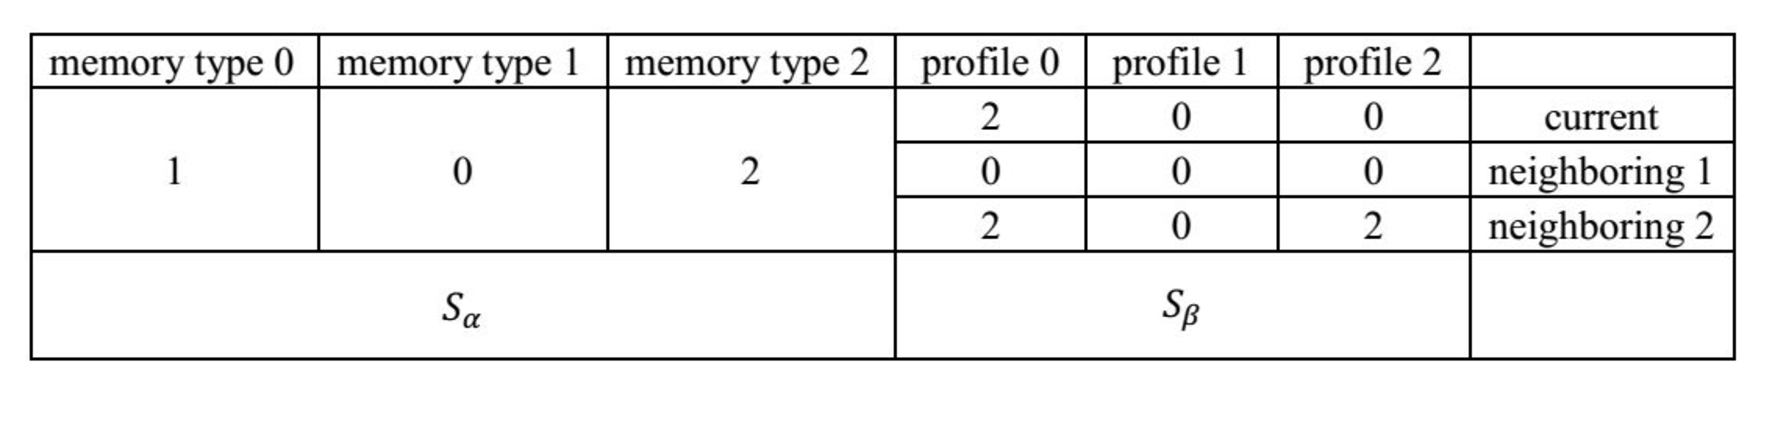
\includegraphics[width=0.7\textwidth]{sa_beta_neigh_example}
			\caption{Neighboring Solutions Example for $SA_{\beta}$}
			\label{fig:sa_beta_neigh_example}
		\end{center}
	\end{figure}		
	
	Algorithm \ref{algo:neighbor_beta} shows the
	pseudo-code of $Neighbor_{\beta}()$. In the algorithm, $S_{\alpha}$ is a solution of
	$SA_{\alpha}$. $memtypes_{allocated}$ is the set of allocated memory types in $S_{\alpha}$.
	$S_{\beta,curr}$ and $S_{\beta,neigh}$ are the current and neighboring solutions
	of $SA_{\beta}$. The method $ConstraintsCheck_{\beta}$ is also used to check whether
	$S_{\beta,neigh}$ satisfy the $Constraint_{\beta}$. It is similar to \ref{algo:constrain_check_1}
	discussed in Section \ref{sec:stage_1}. The only difference is that $ConstraintsCheck_{\beta}$
	does examines the area constraint.
	\setlength{\textfloatsep}{0.2cm}
\begin{algorithm2e}[h]
	\KwIn{$S_{\alpha},S_{\beta,curr}$}
	\KwOut{$S_{\beta,neigh}$}
	create a new solution $S_{\beta,neigh}$\;
	\While{$ConstraintsCheck_{\beta}$($S_{\beta,neigh}$) is false}
	{
		$S_{\beta,neigh}=S_{\beta,curr}$\;
		randomly selecte an element $element_{i}$ in $S_{\beta,neigh}$\;
		identify the set of allocated memory types $memtypes_{allocated}$ in $S_{\alpha}$\;
		randomly selecte an memory type $memtype_{j}$ in $memtypes_{allocated}$\;
		$element_{i}$ = index of $memtype_{j}$ in $S_{\alpha}$\;
	}
	\Return $S_{\beta,neigh}$ \;
	\caption{$Neighbor_{\beta}()$}
	\label{algo:neighbor_beta}
\end{algorithm2e}
\setlength{\textfloatsep}{0.2cm}


	
	In $SA_{\beta}$, the solution cost is still the memory power consumption that can be calculated
	according to the power model.
	In $SA_{\alpha}$, there is no real cost for the its solution $S_{\alpha}$ because $S_{\alpha}$
	only contains the information about the allocation. Thus, the memory power consumption can not
	be calculated according to the power model. However, the cost function of $SA_{\alpha}$ evokes
	the procedure of $SA_{\beta}$. Then $SA_{\beta}$ optimizes the binding based on the current 
	solution of $SA_{\alpha}$. After $SA_{\beta}$ terminates, it provides a binding with the
	minimum memory power consumption to the cost function of $SA_{\alpha}$. $SA_{\alpha}$ sets
	the minimum power consumption as its solution cost. Figure \ref{fig:nested_call} shows the
	nested simulated annealing procedure. In the figure, $C_{\alpha}$ and $C_{\beta}$ are the
	solution cost for $SA_{\alpha}$ and $SA_{\beta}$ respectively.
	\begin{figure}[h]
		\begin{center}
			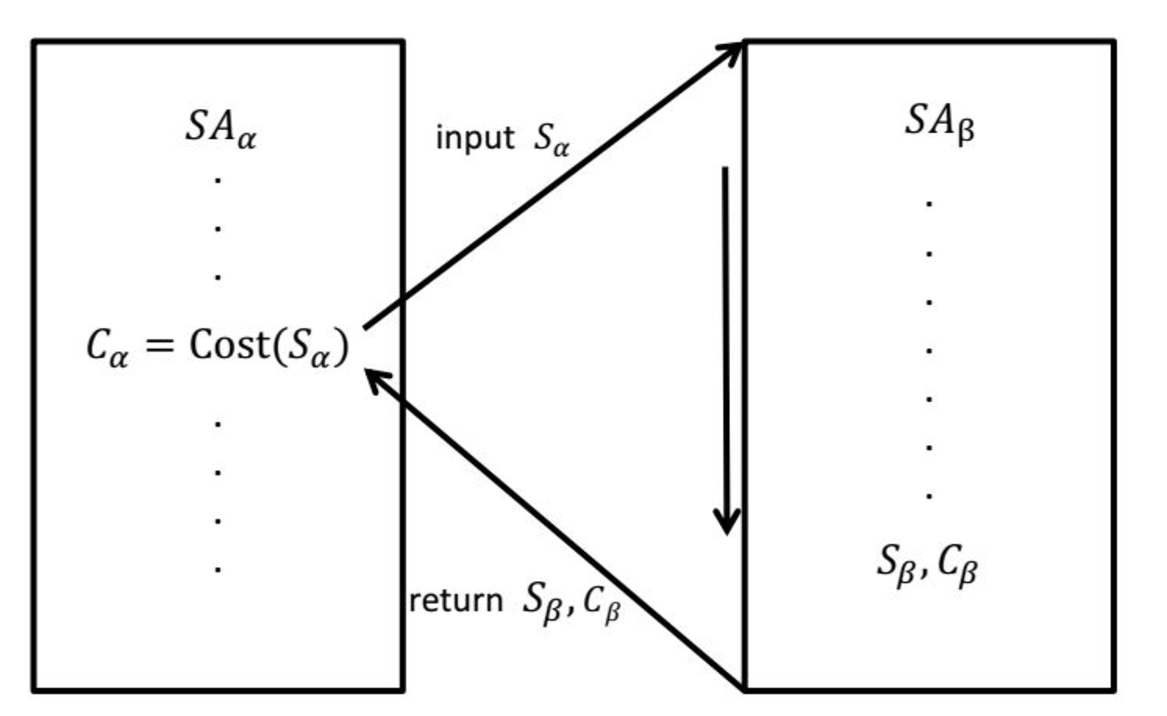
\includegraphics[width=0.7\textwidth]{nested_call}
			\caption{Nested Simulated Annealing Procedure}
			\label{fig:nested_call}
		\end{center}
	\end{figure}

	In this approach, the metropolis criterion and the cooling schedule of both $SA_{\alpha}$
	and $SA_{\beta}$ are the same with the discussion in Section \ref{sec:stage_1}.
	
	For the inner loop termination, Equation \ref{equa:iteration_innerloop} is still used.
	However, the neighborhood size determinations of $SA_{\alpha}$ and $SA_{\beta}$
	are described as following. The neighborhood size
	$Size_{neighbor,\alpha}$ is calculated according to Equation \ref{equa:neighbor_size_a}.
	The length of $S_{\alpha}$ is actually the total number of memory types.
	Because $SA_{\beta}$ is embedded in $SA_{\alpha}$, $Size_{neighbor,\beta}$ is based on
	the solution of $SA_{\alpha}$. It is calculated according to Equation \ref{equa:neighbor_size_b}.
	In the equation, $\lvert memtypes_{allocated} \rvert$ is the number of allocated memory
	types in the current solution of $SA_{\alpha}$. The length of $S_{\beta}$ is actually the
	total number of profiles.
	\begin{equation}
	\label{equa:neighbor_size_a}
		Size_{neighbor,\alpha}=2 \cdot \text{length of } S_{\alpha} 
	\end{equation}
	\begin{equation}
	\label{equa:neighbor_size_b}
		Size_{neighbor,\beta}=\lvert memtypes_{allocated} \rvert \cdot \text{length of } S_{\beta} 
	\end{equation}
	
	For the outer loop termination and determinations of the initial solution and temperature,
	both $SA_{\alpha}$ and $SA_{\beta}$ use the same mechanism introduced in Section
	\ref{sec:stage_1}.
	
	
	
	
	
	